% !TeX spellcheck = en_US
\documentclass[a4paper, 11pt]{article}
\usepackage{layouts} % Feel free to remove this one
\usepackage{amsmath,amsthm,amssymb}
\usepackage[backend=biber, sortcites, citestyle=numeric]{biblatex}
\usepackage[tt=false]{libertine}
\usepackage{libertinust1math}
\usepackage[T1]{fontenc}
\usepackage{enumitem}
\usepackage[top=1in, bottom=1in, left=1.6in, right=1.6in]{geometry}
\usepackage{graphicx} % Required for inserting images
\usepackage{ifthen}
\usepackage{listings}
\usepackage{siunitx-v2}
\usepackage{subcaption}
\usepackage[most]{tcolorbox}
\usepackage{xcolor}
\usepackage{tikz}

\usepackage[colorlinks, linkcolor=black]{hyperref}

\addbibresource{references.bib}

\numberwithin{equation}{section}

\DeclareCaptionFormat{custom}
{%
	{\sf\footnotesize\textbf{#1#2}{#3}}
}
\captionsetup{format=custom}

% Margin paragraphs
\let\oldmarginpar\marginpar
\setlength\marginparwidth{3cm}
\renewcommand{\marginpar}[1]{\oldmarginpar{\flushleft\tiny\sf{#1}}}

% Colors
\definecolor{primary}{HTML}{5080da}
\definecolor{secondary}{HTML}{da8050}

% tikz definitions
\tikzset{leaf node/.style = {rectangle, draw=black, minimum width = 0.5cm, minimum height = 0.5cm}}
\tikzset{internal node/.style = {circle, draw=black, minimum width = 0.5cm}}

% Theorems
\newtcbtheorem{definition}{Definition}{colback=primary!5, colframe=primary, fonttitle=\bfseries}{def}
\newtcbtheorem{alert}{Alert}{colback=secondary!5, colframe=secondary, fonttitle=\bfseries}{alert}

\theoremstyle{definition}
\newtheorem{exercise}{Exercise}[section]

% Code listings

\definecolor{codegreen}{rgb}{0,0.6,0}
\definecolor{codegray}{rgb}{0.5,0.5,0.5}
\definecolor{codepurple}{rgb}{0.58,0,0.82}
\definecolor{backcolour}{rgb}{0.95,0.95,0.92}

\lstdefinestyle{mystyle}{
	backgroundcolor=\color{backcolour},   
	commentstyle=\color{codegreen},
	keywordstyle=\color{magenta},
	numberstyle=\tiny\color{codegray},
	stringstyle=\color{codepurple},
	basicstyle=\ttfamily\footnotesize,
	breakatwhitespace=false,         
	breaklines=true,                 
	captionpos=b,                    
	keepspaces=true,                 
	numbers=left,                    
	numbersep=5pt,                  
	showspaces=false,                
	showstringspaces=false,
	showtabs=false,                  
	tabsize=2
}

\lstset{style=mystyle}

% Custom commands
\newcommand{\Z}{\mathbb{Z}}
\newcommand{\hint}{\textit{Hint:}~}
\newcommand{\inlcd}[1]{\lstinline[language=Python]{#1}}

% inline code blocks
\newcommand\mystrut{\rule[-1pt]{0pt}{.8em}}

\newtcbox{\code}{on line, boxrule=0pt, boxsep=0pt, top=2pt,
	left=2pt, bottom=2pt, right=2pt, colback=gray!25, colframe=white,
	fontupper={\ttfamily\mystrut}}

% Colors
\definecolor{primary}{HTML}{5080da}

% Theorems
\newtcbtheorem{task}{Task}{colback=primary!5,colframe=primary,fonttitle=\bfseries}{task}

% Custom commands
\newcommand{\player}{\texttt{p}}
\newcommand{\fow}{\texttt{*}}
\newcommand{\relic}{\texttt{+}}
\newcommand{\visited}{\texttt{.}}

%%% Local macros
\newcommand{\caret}{\,^\wedge\,}

\title{Programming Lab 02: Collecting Relics}
\author{V. Markos\\Mediterranean College}
\date{\today}

\begin{document}
	%
	\maketitle
	%
	\begin{abstract}
		What is this? Probably an ongoing lab for this course, where you will create simple game in Python. Do not expect spectacular graphics and all that stuff, since this course is not about that, but expect to encounter and attack several data structures and algorithm--related problems as we go into more sophisticate designs for our game. Stay tuned for more\ldots
	\end{abstract}
	%
	%
	%
	\section{Last Time Recap}
	%
	Last time we implemented a game with the following features (at least):
	\begin{itemize}
		\item A customisable game grid, initially covered by a fog of war (i.e., \fow), which could have any of the following sizes:
		\begin{itemize}
			\item $15\times 15$;
			\item $20\times 20$;
			\item $30\times 30$.
		\end{itemize}
		\item A player printed on screen, initially positioned at the bottom left corner of the grid.
		\item Player movement using \texttt{nswe} or \texttt{wasd} keys to move around the grid.
		\item Relevant movement restrictions, i.e., the player cannot cross grid borders (or, movement wraps around the grid, whichever you prefer).
		\item Optionally, you might have also your grid printing over its previous version to avoid overloading the terminal with unnecessary past versions of the grid.
	\end{itemize}
	%
	%
	%
	\section{Hiding Relics}
	%
	So far, our main character can move around the grid exploring the grid, but last time we did not implement something really crucial: lifting the fog of war. Evidently, once our player has passed through a certain grid cell, we should denote this cell as explored, letting the player know that this cell has already been visited. So, here comes your first task for this lab:
	
	\begin{task}{Lifting the FoW}{lifting}
		You should keep track of player movement around the grid and print any already visited cells using a \visited (dot). You should choose an appropriate Python data structure for the visited cells in your grid (take into consideration which operations you will need to perform most often on them). So, each cell might now be in either of the following states:
		\begin{itemize}
			\item Unexplored, covered by the FoW, indicated by a \fow.
			\item Explored, indicated by a dot (\visited).
			\item Containing the player, indicated by a \player.
		\end{itemize}
		For instance, a small game grid where the player has explored some of its bits is shown in Figure~\ref{fig:explored grid}.
	\end{task}
	
	\begin{figure}[!tb]
		\centering
		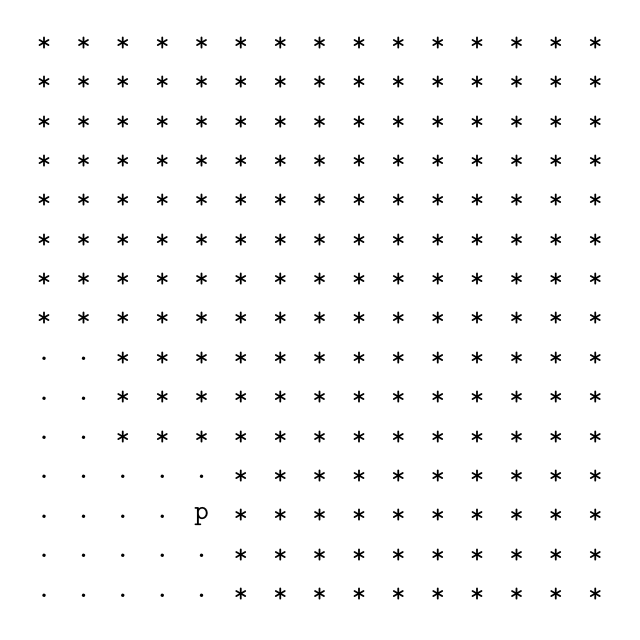
\begin{tikzpicture}
			\foreach \i in {0,...,14} {
				\pgfmathsetmacro{\xcoord}{0.5*\i}
				\foreach \j in {0,...,14} {
					\pgfmathsetmacro{\ycoord}{0.5*\j}
					\ifthenelse{\i=4\AND\j=2}{
						\node (\i\j) at (\xcoord,\ycoord) {\player};
					}{
						\ifthenelse{{\i<5\AND\j<4}\OR{\i<2\AND\j<7}}{
							\node (\i\j) at (\xcoord,\ycoord) {\visited};
						}{
							\node (\i\j) at (\xcoord,\ycoord) {\fow};
						}
					}
				}
			}
		\end{tikzpicture}
		\caption{A small, $15\times 15$ grid where the player has explored some of its parts. Explored parts are indicated by a ``\visited''.}
		\label{fig:explored grid}
	\end{figure}
	
	Leaving Task~\ref{task:lifting} behind us, we move to a more juicy part of our game: hiding relics. To this end, let us first sketch a rough idea on how things should work:
	\begin{itemize}
		\item Our main character wanders around the grid, exploring the world.
		\item At random places throughout the grid, collectible relics are hidden.
		\item Whenever the player encounters a relic, the relic is considered as collected and a point is awarded to the player (we might make use of this point system in subsequent labs somehow).
	\end{itemize}
	
	Bearing the above in mind, here comes your next task:
	
	\begin{task}{Placing Relics}{placing relics}
		Implement any relevant functionality that will allow you to place some relics on the game grid. As a rule of thumb, place as many relics as the number of rows / columns for each size of the grid. So, in a $15\times 15$ grid you should place 15 relics, on a $20\times 20$ grid place 20 relics, etc. The relics should be placed \textbf{at random} so starting a new game from scratch results to different relic positioning (to avoid players reverse engineering our game).
		
		Some things to take into account:
		\begin{itemize}
			\item You can use Python's \texttt{random} module and all relevant functions it offers for randomly generating numbers.
			\item There are several pitfalls you will need to \textbf{avoid}, the most common probably being \textbf{generating less relics} than you might think (if you do not utilise \texttt{random} utilities appropriately).
			\item Choose an appropriate representation for your relics in terms of Python data structures! Bear in mind that in subsequent tasks you will need to frequently check whether a relic is in a certain cell or not!
		\end{itemize}
		
		In order to facilitate debugging, you can create a function that prints a grid containing only the relics, e.g., as shown in Figure~\ref{fig:relics}.
	\end{task}
	
	\begin{figure}[!tb]
		\centering
		\begin{tikzpicture}
			\foreach \i in {0,...,14} {
				\pgfmathsetmacro{\xcoord}{0.5*\i}
				\foreach \j in {0,...,14} {
					\pgfmathsetmacro{\ycoord}{0.5*\j}
					\foreach \li/\lj in {4/2,6/1,14/3, 5/9, 9/7, 8/6} {
						\ifthenelse{{\i=\li\AND\j=\lj}}{
							\node (\i\j) at (\xcoord,\ycoord) {\relic};
						}{
							\node (\i\j) at (\xcoord,\ycoord) {\visited};
						}
					}
				}
			}
		\end{tikzpicture}
		\caption{Debugging relics positioning, just with fewer relics than expected. In the above, relics are denoted by a ``plus'' (\relic).}
		\label{fig:relics}
	\end{figure}
	
	%
	%
	%
	\section{Collecting Relics}
	%
	Having placed our relics on the map, we should now implement any infrastructure related to actually collecting relics.
	\begin{task}{Collecting Relics}{collecting relics}
		Implement any required functionality regarding collecting relics. Your implementation should address, at least, the following:
		\begin{itemize}
			\item Whenever the main character moves onto a relic, it should be collected, keeping track of how many relics have been collected so far.
			\item The player should be informed about such events by an appropriate message on screen.
			\item The total number of collected relics should be displayed at some reasonable place on the game's screen --- this will vary depending on whether you print every version of the game grid or overwrite previous ones.
		\end{itemize}
	\end{task}
	
	What if our player collects all available relics? For now this will be the ``Game Over'' scenario of our game. So, here comes your last (small) task for today:
	\begin{task}{Game Over}{game over}
		Implement any game over related functionality that informs the player that they have collected all collectible relics, while you should also offer them the choice to start a new game or quit the game at all.
	\end{task}
	%
	%
	%
	\section{Further Considerations}
	%
	One possible twist regarding relic collection could be the introduction of relics of various values. For instance, a simple relic could equal 1 point while a super--relic could offer 3 points.
	
	\begin{task}{Super Relics}{super relics}
		Implement a differentiated scoring regarding relics. You should offer at least two different relic types (feel free to improvise regarding their names). This might also affect the way a game ends. For instance, in a small, $15\times 15$, grid, the primary objective might be to collect 10 points, be it by collecting 10 simple relics or 5 super relics or a combination of those, and, possibly, even more complex relic types. Explain your design choices appropriately!
	\end{task}
	
	What if a player does not want to collect a relic? For instance, some players might prefer to first explore the game map and then collect any relics they encounter following an optimal path for doing so. So, here comes another interesting task:
	
	\begin{task}{Dropping Relics}{dropping relics}
		Allow players to drop relics, in the sense of ignoring relics whenever they encounter them. This can be implemented as a short in--game dialogue that is displayed below the game grid, where the player provides some sort of Y/N (yes/no) response to a simple prompt. You can also keep track of rejected relics and any relevant statistics.
	\end{task}
	%
	%
	%
\end{document}
